\documentclass[tikz,convert,crop,boder=100px]{standalone}
% vim:noet:sts=2:ts=2:sw=2:smarttab:tw=120
\usepackage{pgfplots}
\usetikzlibrary{arrows,shapes,positioning,calc}

\begin{document}
	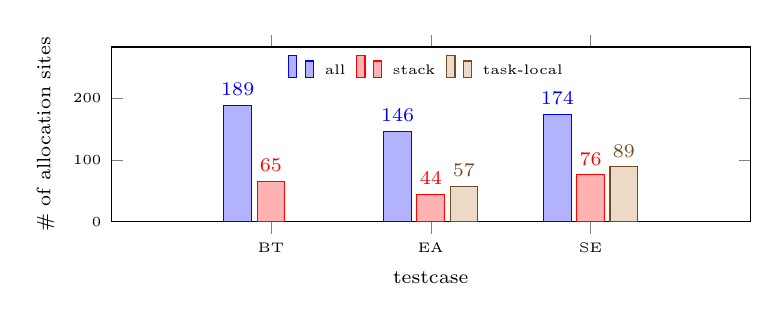
\begin{tikzpicture}[font=\scriptsize]
		\begin{axis}[
			width=.8\textwidth,
			height=3.8cm,
			ybar,
			%bar width=15pt,
			ylabel=\# of allocation sites,
			xlabel=testcase,
			enlarge x limits=0.5,
			ymin=0,
			enlarge y limits={value=0.5,upper},
			symbolic x coords={BT, EA, SE},
			xtick=data,
			nodes near coords,
			nodes near coords align={vertical},
			legend style={draw=none, fill=none, at={(0.5, 0.99)}, anchor={north}, legend columns=-1},
			legend cell align=left,
			label style={font=\scriptsize},
			tick label style={font=\tiny},
			legend style={font=\tiny}
		]
			% all allocations
			\addplot coordinates {(BT, 189) (EA, 146) (SE, 174)};
			\addlegendentry{\;all\;}
			\addplot coordinates {(BT, 65) (EA, 44) (SE, 76)};
			\addlegendentry{\;stack\;}
			\addplot coordinates {(EA, 57) (SE, 89)};
			\addlegendentry{\;task-local\;}
		\end{axis}
	\end{tikzpicture}
\end{document}
